\documentclass[12pt]{report}
\usepackage{inputenc}
\usepackage{graphicx}
\graphicspath{{./images/}}
\usepackage{geometry}
\usepackage{amsmath}
\usepackage{amssymb}

\usepackage{listings}
\usepackage{listings}
\usepackage{xcolor}

\definecolor{codegreen}{rgb}{0,0.6,0}
\definecolor{codegray}{rgb}{0.5,0.5,0.5}
\definecolor{codepurple}{rgb}{0.58,0,0.82}
\definecolor{backcolour}{rgb}{0.95,0.95,0.92}

\lstdefinestyle{mystyle}{
    backgroundcolor=\color{backcolour},   
    commentstyle=\color{codegreen},
    keywordstyle=\color{magenta},
    numberstyle=\tiny\color{codegray},
    stringstyle=\color{codepurple},
    basicstyle=\ttfamily\footnotesize,
    breakatwhitespace=false,         
    breaklines=true,                 
    captionpos=b,                    
    keepspaces=true,                 
    numbers=left,                    
    numbersep=5pt,                  
    showspaces=false,                
    showstringspaces=false,
    showtabs=false,                  
    tabsize=2
}

\lstset{style=mystyle}


\title{MATH40011 Calculus for JMC 
 \\ Revision Note}
\author{Feifan Fan}


\begin{document}
\maketitle
\tableofcontents

\chapter{Differentiation}

\section{Basic Differentiation}

\subsection{Parametric Graph Sketching}

\emph{We are going to sketch a parametric curve $x = f(t)$, $y = g(t)$.}
\newline

\noindent Some basic rules:
\begin{itemize}
    \item Try to find the function $y = h(x)$ between $y$ and $x$
    
    and try to determine the symmetry of the curve: 
    
    i.e. determine whether $h(x) = h(-x)$ 
    
    \emph{(even function, curve is symmetrical about y axis)}

    or $h(x) + h(-x) = 0$ 
    
    \emph{(odd function, curve is symmetrical about the origin)}
    
    or if we have $y^{2} = t(x) \implies y = \pm \sqrt{t(x)}$

    \emph{(not a function, but curve is symmetrical about the x axis}

    \emph{since a value of x points to two values with opposite signs)}
    \item Find the zero points of the curve:
    
    Calculate the value of $t$ such that $y = g(t) = 0$, 
    and calculate the correspnding value of x 
    to get the zero point $(x, 0)$
\end{itemize}
Some special rules for the parametric curves:
\begin{itemize}
    \item Determine when the tangent line to the curve is \emph{horizontal} and \emph{vertical}:
    \newpage
    \emph{Horizontal:} find the value of t such that
    $$
    \frac{dy}{dx} = \frac{\frac{dy}{dt}}{\frac{dx}{dt}} = 0
    $$
     \indent Hence, the tangent is horizontal if
     $$
    \frac{dy}{dt} =  g'(t) = 0 \text{ and }\frac{dx}{dt} = f'(t) \neq 0
     $$
     \emph{Vertical:} find the value of t such that
     $$
     \frac{dy}{dx} = \frac{\frac{dy}{dt}}{\frac{dx}{dt}} = \pm \infty
     $$
     \indent Hence, the tangent is horizontal if
     $$
    \frac{dy}{dt} =  g'(t) \neq 0\text{ and } \frac{dx}{dt} = f'(t) = 0
     $$
    \item Determine at which points is the tangent line to the curve parallel to $y = x$:
    \newline Since for the line $y = x$, $\frac{dy}{dx} = 1$,

    Therefore, if the tangent line is parallel to y = x, 
    $$
    \frac{dy}{dx} = \frac{\frac{dy}{dt}}{\frac{dx}{dt}} = 1
    $$
    \newline Hence, we have 
    $$
    g'(t) = \frac{dy}{dt} = \frac{dx}{dt} = f'(t)
    \text{ where } g'(t) = f'(t) \neq 0$$
    \item Find the limit of the gradient when t is close to 0:
    \newline  $$
    \lim_{t \to 0^+} \frac{dy}{dx} = \lim_{t \to 0^+} \frac{\frac{dy}{dt}}{\frac{dx}{dt}}
    \text{ and }
    \lim_{t \to 0^+} \frac{dy}{dx} = \lim_{t \to 0^+} \frac{\frac{dy}{dt}}{\frac{dx}{dt}}
    $$
    \item Similarly, find the limit of the gradinet when t tends to $\pm \infty$:
    \newline $$
    \lim_{t \to \pm \infty} \frac{dy}{dx} = \lim_{t \to \pm \infty} \frac{\frac{dy}{dt}}{\frac{dx}{dt}}
    $$
    
    In conclusion, we can combine the elements above and find the "dirction" of $t$ to sketch the parametric curve. 
\end{itemize}
 
\newpage
\emph{Example: Sketch the curve}
$$
\left\{\begin{array}{ll}
x = t^2 
\\ y = t^3 - t
\end{array}\right.
$$
\indent in the cartesian plane.

\begin{enumerate}
    \item Firstly we know that $y = t^3 - t = t(t^2 - 1) = t(x - 1)$.
    \newline And we squared y to get:
    $$
    y^2 = t^2(x - 1)^2 = x(x - 1)^2
    $$
    Therefore, 
    $$
    y = \pm \sqrt{x(x - 1)^2}
    $$
    Clearly this curve is symmetrical about x axis. \emph{(symmetry $\checkmark$)}
    \item Then we let $y = 0$ to find the zero point(s), i.e.
    $$
    y = t^3 - t = t(t^2 - 1) = 0
    $$
    So we have:
    $$
    t = 0 \text{ or } t^2 = 1
    $$
    Therefore, $$
    t = 0 \text{ or } \pm 1
    $$
    We substitute the value of $t$ in the expression of $x$, and get:
    $$
    \begin{array}{lll}
        t = 0, & x = 0 & y = 0 \\
        t = 1, & x = 1 & y = 0 \\
        t = -1, & x = 1 & y = 0 \\
    \end{array}
    $$
    Therefore, the zero points of this parametric curve is $(0, 0) \text{ and } (1, 0)$.
    
    \emph{(zero points \checkmark)}

    \item Next we need to determine when the tangent of the curve is horizontal 
    (also determine the local extrema) and when it is vertical:

    \emph{Horizontal:} We can easily calculate that $\frac{dx}{dt} = 2t$ and $\frac{dy}{dt} = 3t^2 - 1$.

    Therefore, let $\frac{dy}{dt} = 3t^2 - 1 = 0$:
    
    We then have:
    $$
    \begin{array}{l}
        t^2 = \frac{1}{3} \\
        t = \pm \frac{\sqrt{3}}{3}
    \end{array}
    $$
    We confirmed that when $\frac{dy}{dt} = 0$, $\frac{dx}{dt} \neq 0$.

    Therefore, the points are at:
    $$
    \begin{array}{lll}
        t = \frac{\sqrt{3}}{3}, & x = \frac{1}{3} & y = -\frac{2 \sqrt{3}}{9} \\
        t = -\frac{\sqrt{3}}{3}, & x = \frac{1}{3} & y = \frac{2 \sqrt{3}}{9} \\
    \end{array}
    $$
    i.e. The (local extrema) points are $(\frac{1}{3}, -\frac{2\sqrt{3}}{9}) \text{ and } (\frac{1}{3}, \frac{2\sqrt{3}}{9})$.
    
    Since 
    $$
    \begin{array}{l}
        \frac{d^2y}{dx^2} = \frac{d}{dx}(\frac{dy}{dx}) = \frac{d}{dx}(\frac{3t^2 - 1}{2t})\\\\
        =\frac{d}{dt}(\frac{3}{2}t - \frac{1}{2t})\frac{dt}{dx}
        = \frac{1}{2t}(\frac{3}{2} + \frac{1}{2t^2}) 
        = \frac{3}{4t} + \frac{1}{8t^3}
    \end{array}
    $$
    Clearly, we could see that when $t$ is negative, so is the value of $\frac{d^2y}{dx^2}$. 
    
    In this case, 
    $(\frac{1}{3}, \frac{2\sqrt{3}}{9})$ is the local maximum point.

    Similarly,
    $(\frac{1}{3}, -\frac{2\sqrt{3}}{9})$ is the local minimum point.

    \emph{Vertical:} 
    
    Just like how we deal with the points with horizontal tangents, 
    let $\frac{dx}{dt} = 2t = 0$:

    Clearly, the only answer that satisfies the equation is $t = 0$.

    Therefore, $(0, 0)$ is the point where the tangent is vertical.

    \emph{(special points with horizontal/vertical tangents \checkmark)}
    \item Also we need to determine when the tangent is parallel to y = x:
    
    Let $\frac{dy}{dt} = \frac{dx}{dt}$, i.e. $2t = 3t^2 - 1 \implies 3t^2 - 2t - 1 = 0$:

    Then we have $$
    \begin{array}{ll}
        (t - 1)(3t + 1) = 0\\
        t_1 = 1 \text{ or } t_2 = -\frac{1}{3}
    \end{array}
    $$Therefore, the points we required are:$$
    \begin{array}{lll}
        t = 1,  & x = 1 & y = 0 \implies (1, 0) \\
        t = -\frac{1}{3} & x = \frac{1}{9} & y = \frac{8}{27} \implies (\frac{1}{9}, \frac{8}{27})
    \end{array}
    $$
    \item Finally we find the behaviour of the gradient, when it is close to $0$ 
    
    and/or it tends to $\pm \infty$:

    $$
    \lim_{t \to 0^+} \frac{dy}{dx} = \lim_{t \to 0^+} \frac{3t^2 - 1}{2t}
    $$

    \item In conclusion, we combine the elements together and plot the graph below:
    \begin{figure}[h]
        \centering
        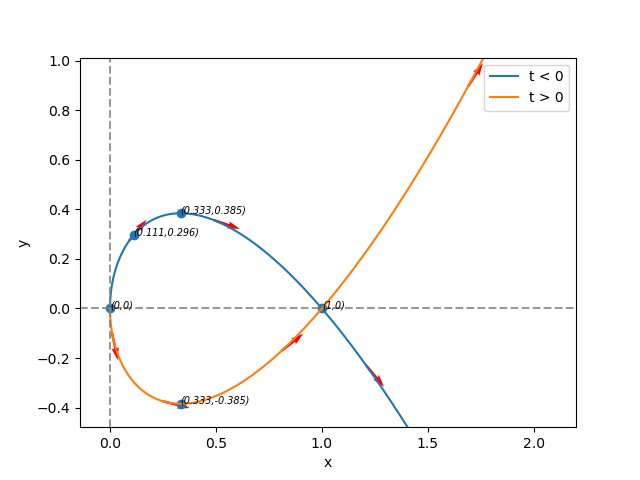
\includegraphics[scale = 0.6]{parametric-curve-sketching.png}
        \caption{the parametric curve with direction of gradients}    
    \end{figure}
\end{enumerate}
    


\section{Differentiability \& Continuity of a function}


\appendix

\chapter{Code for Graph Sketching}
This chapter contains all the code for demonstrative graph sketching in the notes.
Most of the code is written in Python, a few lines of code are in Matlab, maybe there are some code in R as well.
\section{Parametric Curve Sketching}
This is the code for sketch the parametric curve in chapter():

$$
\left\{\begin{array}{ll}
x = t^2 
\\ y = t^3 - t
\end{array}\right.
$$ in the cartesian plane, written in Python:

\lstinputlisting[language = Python]{parametric-curve.py}

\section{False Position}



\section{Starting the Appendices}
Actually, using appendices is quite simple.  Immediately after the end
of the last chapter and before the start of the first appendix, simply
enter the command \verb|\appendix|.  This will tell \LaTeX~to change
how it interprets the commands \verb|\chapter|, \verb|\section|,
\textit{etc.}

Each appendix is actually a chapter, so once the \verb|\appendix|
command has been called, start a new appendix by simply using the
\verb|\chapter| command.

Note that the \verb|\appendix| command should be called only
once--not before the start of each appendix.

All the fancy referencing and tools still work.
You only need to add the appendix command and all will be as it should be.

\chapter{Another Appendix}


\end{document} 